% TEMPLATE for Usenix papers, specifically to meet requirements of
%  USENIX '05
% originally a template for producing IEEE-format articles using LaTeX.
%   written by Matthew Ward, CS Department, Worcester Polytechnic Institute.
% adapted by David Beazley for his excellent SWIG paper in Proceedings,
%   Tcl 96
% turned into a smartass generic template by De Clarke, with thanks to
%   both the above pioneers
% use at your own risk.  Complaints to /dev/null.
% make it two column with no page numbering, default is 10 point

% Munged by Fred Douglis <douglis@research.att.com> 10/97 to separate
% the .sty file from the LaTeX source template, so that people can
% more easily include the .sty file into an existing document.  Also
% changed to more closely follow the style guidelines as represented
% by the Word sample file. 

% Note that since 2010, USENIX does not require endnotes. If you want
% foot of page notes, don't include the endnotes package in the 
% usepackage command, below.

% This version uses the latex2e styles, not the very ancient 2.09 stuff.
\documentclass[letterpaper,twocolumn,10pt]{article}
\usepackage{usenix,epsfig}
\usepackage{listings}
\usepackage{color}
\usepackage{subcaption}
\usepackage{tikz}
\usepackage{hyperref}
\usetikzlibrary{arrows,automata}

\definecolor{mygray}{rgb}{0.5,0.5,0.5}
\lstset{frame=tb,
  language=Ruby,
  basicstyle={\scriptsize\ttfamily},
  breaklines=true,
  captionpos=b,
  numbers=left,
  numbersep=5pt,
  numberstyle=\tiny\color{mygray},
  xleftmargin=2em,
frame=l,
framexleftmargin=1.5em
}

\usepackage[font=footnotesize,labelfont=bf]{caption}

\begin{document}

%don't want date printed
%\date{}

%make title bold and 14 pt font (Latex default is non-bold, 16 pt)
%\title{\Large \bf Working Titles: Layering is dead, long live layering!
%Layering is for the faint of heart; Layer Slayer: Dynamic Optimization, like a True Player.}
\title{DeclStore: Layering is for the Faint of Heart}

%for single author (just remove % characters)
\author{
    {\rm Noah Watkins, Michael A. Sevilla, Ivo Jimenez, Kathryn Dahlgren,}\\
{\rm Peter Alvaro, Shel Finkelstein, Carlos Maltzahn}\\
The University of California, Santa Cruz\\
\{jayhawk, msevilla, ivo, carlosm\}@soe.ucsc.edu, \{kmdahlgr, palvaro, shel\}@ucsc.edu
} % end author

\maketitle

% Use the following at camera-ready time to suppress page numbers.
% Comment it out when you first submit the paper for review.
\thispagestyle{empty}
\pagenumbering{gobble}


%\subsection*{Abstract}
%Your Abstract Text Goes Here.  Just a few facts.
%Whet our appetites.

\section{Introduction}
\label{sec:intro}

Popular storage systems support diverse storage abstractions by
providing important disaggregation benefits. Instead of maintaining
a separate system for each abstraction, \emph{unified} storage
systems, in particular, support standard file, block, and object abstractions so the same
hardware can be used for a wider range and a more flexible mix of applications. 
As large-scale unified storage systems continue to evolve to meet the requirements 
of an increasingly diverse set of applications and next-generation hardware, \emph{de jure}
approaches of the past---based on standardized interfaces---are giving way to
domain-specific interfaces and optimizations. While promising, the ad-hoc strategies characteristic of 
current approaches to co-design are untenable.

The standardization of the POSIX I/O interface has been a major success. General adoption
has allowed application developers to avoid vendor lock-in and encourages storage system
designers to innovate independently. However, large-scale storage systems are generally dominated 
by proprietary offerings, preventing exploration of alternative
interfaces when the has presented itself. An increase in the number of special-purpose storage systems characterizes recent history
in the field, including the emergence of high-performance, and highly modifiable, open-source storage systems, 
which enable system changes without of vendor lock-in. Unfortunately, evolving storage system
interfaces is a challenging task requiring domain expertise, and is predicated on the willingness of
programmers to forfeit the protection from change afforded by narrow
interfaces.

Malacology~\cite{sevilla:eurosys17} is a recently proposed storage system that
advocates for an approach to co-design called \emph{programmable storage}. The
approach exposes low-level functionality as reusable building
blocks, allowing developers to custom-fit their applications to take advantage
of the existing code-hardened capabilities in underlying system, and avoid
duplication of complex and error-prone services. By recombining existing
services in the Ceph storage system~\cite{weil:osdi2006-ceph}, Malacology
demonstrated how two
real-world services, a distributed shared-log and a file system metadata load
balancer, could be constructed using a `dirty-slate` approach. Unfortunately,
an ad-hoc approach can be difficult to effectively reason about and manage.

Despite the benefits of the approach demonstrated by Malacology, the technique
requires navigation of
a complex design space and simultaneously addressing often orthogonal
concerns (e.g. functional correctness, performance, and fault-tolerance).
Worse still, the availability of domain expertise required to build a performant interface is not a fixed or reliable resource. 
As a result, the interfaces built with Malacology are sensitive to evolving
workloads, and changes to the underlying hardware and software systems,
necessitating burdensome maintenance overhead.

To address these challenges, we advocate for the use of high-level declarative
languages (e.g. Datalog) as a means of programming new storage system
\emph{interfaces}.  By specifying the functional behavior of a storage interface once
in a relational (or algebraic) language, optimizers built around cost models
can explore a space of
functionally equivalent physical implementations. Much like query planning and
optimization in database systems, this approach will logically differentiate
correctness from performance, and protect higher-level services from lower-level
system changes. However, despite the parallels with database systems, this
paper demonstrates, and begins to address, fundamental differences in the
optimization design space.

In this paper we demonstrate the challenge of programmable storage by showing
the sensitivity of domain-specific interfaces to changes in the underlying
system. We then show that the relational model is able to capture the
functional behavior of a popular shared-log service, and finally we explore
additional optimizations capable of expanding the space of
possible implementations.

\section{Programmable Storage}
\label{sec:progly}

Common workarounds when application requirements are not met
by an underlying storage system roughly fall into three categories:

{\bf ``Bolt-on services''} improve performance
or enable new features, but come at the expense of additional hardware, software
sub-systems, and dependencies that must be managed, as well as trusted.
For instance, such classes of limitations inspired many extensions to Hadoop
~\cite{bu:vldb2010-haloop, ekanayake:hpdc2010-twister,
ekanayake:escience2008-eglmapreduce, mihailescu:hotstorage2012-mixapart}.

{\bf Application changes} introduce data management intelligence or integrate
domain-specific middleware into an application.  When application changes
depend on non-standard storage semantics (e.g. relaxed POSIX file I/O or
MPI-IO hints) the resulting coupling can be fragile.  For example, both
SciHadoop~\cite{buck:hpc2011-scihadoop} and
Rhea~\cite{gkantsidis:nsdi2013-rhea} do an excellent job of partitioning data
in Hadoop applications, but may not withstand the test of time for future
workloads, since the partitioning is specific to the use case. Approaches to
I/O optimization in middleware (e.g.  MPI-IO) take advantage of an
application's structured and partitioned data model, but face portability
challenges when mapping parallel I/O onto a bytestream. The challenge is, in
part, due to the wide range of optimization strategies that are dependent on
low-level storage system \emph{magic numbers} for optimal data partitioning,
distribution, and alignment. The PLFS file system takes an approach of
virtualizing the POSIX byte stream over a set of logs to address this
issue~\cite{plfs}.

{\bf Storage system modifications} are often a last resort because such
heavyweight solutions range from merely changing the underlying system to
designing entirely new systems. This approach requires at a minimum, a certain level of
access to modify the system, significant cost, domain knowledge, and extreme care when building or
modifying critical software that can take years of code-hardening to trust.
For example, HDFS fails to meet many needs of metadata-intensive
workloads~\cite{shvachko:login2012-hdfs-scalability}.  This has lead to
modifications to its architecture and API~\cite{balmin:sigmod2012-clydesdale}
to improve performance.

Rather than relying on storage systems or applications to change, Malacology
exposes data management services already present in the underlying system,
which can be re-used to avoid code duplication and reliance on external
services.

\subsection{The Malacology Approach}
\label{mala}

Malacology is a prototype programmable storage system based on Ceph that
improves the development experience of co-designing applications and storage
systems by exposing common internal storage services for
re-use~\cite{sevilla:eurosys17}. Figure~\ref{fig:malacology} shows the
architecture of Malacology, along with the set of services that are exposed,
such as domain-specific object interfaces, cluster-level metadata management,
and load-balancing. While Ceph natively exposes file, block, and object
abstractions, Malacology demonstrates the construction of two real-world
services using only the composition of existing interfaces present in Ceph.

\begin{figure}[t]
\centering
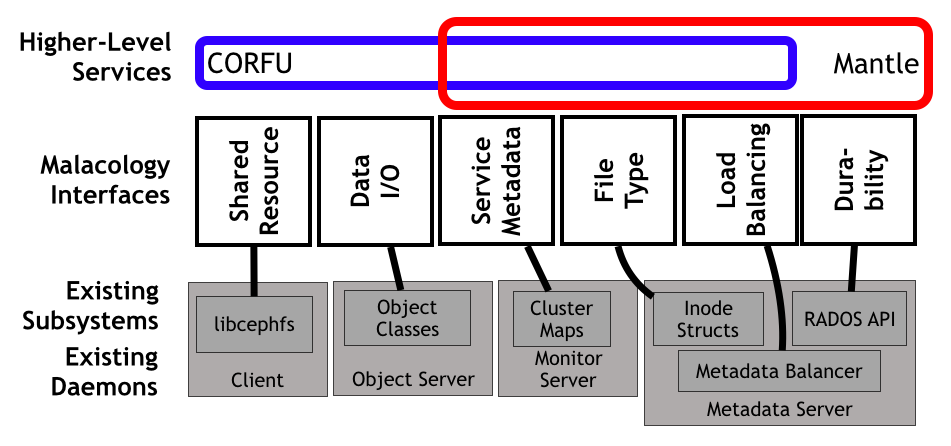
\includegraphics[width=1.0\linewidth]{implementation-overview.png}
\caption{Malacology implementation in Ceph. Existing sub-systems are composed
    to form new services and application-specific optimizations.}
\label{fig:malacology}
\end{figure}

One of these synthesized interfaces is a high-performance distributed
shared-log
based on the CORFU protocol~\cite{balakrishnan:nsdi12}.  While CORFU can
be a stand-alone system, Malacology is capable of instantiating the same storage
abstraction and approximating the same optimizations. High-performance in CORFU
is achieved in part through the use of a soft-state network-attached counter.
Malacology approximates this optimization using the capability-based caching
mechanisms in the Ceph distributed file system, modeling the counter as a
shared resource (i.e. file metadata). Additionally, the co-designed device
interfaces used in CORFU are critical to the safety of the protocol, and are
replicated in Ceph using custom software-based interfaces to storage objects.

While powerful, storage interface construction in Malacology (Data I/O interface in
Figure~\ref{fig:malacology}) is a double-edged
sword. The narrowly-defined interfaces dominating systems today have been a
boon to developers by limiting the size of the design space where applications
couple with storage, allowing systems to evolve independently. Programmable
storage lifts the veil on the system and, with it, forces developers of
higher-level services to confront a large and expanding set of possible
designs.

\section{Design Space}
\label{sec:dspace}

The narrow interface exposed by storage systems has been a boon in allowing
systems and applications to evolve independently, in effect limiting the size
of the design space where applications couple with storage. Programmable
storage lifts the veil on the system, and with it, forces developers of higher-level services
to confront a large and expanding set of possible designs.

In this section we elucidate the matter of design space size and complexity in
programmable storage. We report on our experience building and optimizing
\emph{multiple} functionally equivalent implementations of the CORFU protocol
in Ceph, demonstrating that static selection of optimization strategies and tuning
decisions can lead to performance portability challenges in programmable
storage sytems.

\subsection{System Tunables and Hardware}

A recent version of Ceph (v10.2.0-1281-g1f03205) has 994 tunables parameters,
where 195 of them pertain to the object server itself and 95 of them focus on
low-level storage abstractions built on XFS or BlueStore.  Ceph also has
tunables for the subsystems it uses, like LevelDB (10 tunables), RocksDB (5
tunables), its own key-value stores (5 tunables), its object cache (6
tunables), its journals (24 tunables), and its other optional object stores
like BlueStore (49 tunables).  Auto-tuning~\cite{behzad:sc2013-autotuning}
techniques have been applied to systems with a large space of parameters with
limited success, but the challenge is exacerbated in the context of
application-specific modifications and workloads that change dynamically.

{\bf Hardware.} Ceph is designed to run on a wide variety of commodity
hardware as well as new NVMe devices. All these devices have their own set of
characteristics and tunables (e.g., the IO operation scheduler type). In our
experiments, we tested SSD, HDDs, NVMe devices and discovered a wide range of
behaviors and performance profiles. While we generally observe the expected
result of faster devices resulting in better application performance, choosing
the best implementation strategy is highly dependent on hardware. The changes
in Ceph required to fully exploit the performance profile of NVMe, persistent
memory, and RDMA networks will likely result in new design trade-offs for
application-specific interface designs.

\textbf{Takeaway:} Evolving hardware and system tunables present a challenge
in optimizing systems, even in static cases with fixed workloads. Programmable
storage approaches that introduce application-specific interfaces that are
sensitive to changes in workloads and the cost models of low-level interfaces
that are subject to change  greatly increase the design space and set of
concerns to be addressed by programmers.

\subsection{Software}

The primary source of complexity in large storage systems is unsurprisingly
the vast amount of software written to handle challenges like fault-tolerance
and consistency in distributed heterogeneous environments. We have found that
even routine upgrades can cause performance regressions that introduce
challenges for adopters of a programmable storage approach to development.

The CORFU protocol stripes a log across a cluster of storage
devices that each expose a custom 64-bit write-once address space for reading
and writing log entries. While this interface can be built directly into flash
devices~\cite{wei:systor13}, we constructed four different versions in Ceph
each as a software abstraction over the existing object interface.
Each of our software-based implementations differ in their optimization
strategy of utilizing internal system interfaces. For instance one
implementation uses a key-value interface to manage the address space index
and entry data, while another implementation stores the entry data using a
byte-addressable interface. 

Figure~\ref{fig:phy-design} shows the append throughput of four such
implementations run on two versions of Ceph from 2014 and 2016. The first
observation to be made is that performance in general is significantly better
in the newer version of Ceph. However, what is interesting is the relationship
between the implementations. Run on a version of Ceph from 2014, the top two
implementations perform with nearly identical throughput, but have strikingly
different implementation complexities. The performance of the same
implementations on a newer version of Ceph illustrate a challenge: given a
reasonable choice of a simpler implementation in 2014, a storage interface
will perform worse in 2016, requiring significant rework of low-level
interface implementations.

\begin{figure*}[t]
    \centering
    \begin{subfigure}[b]{.33\linewidth}
        \centering
        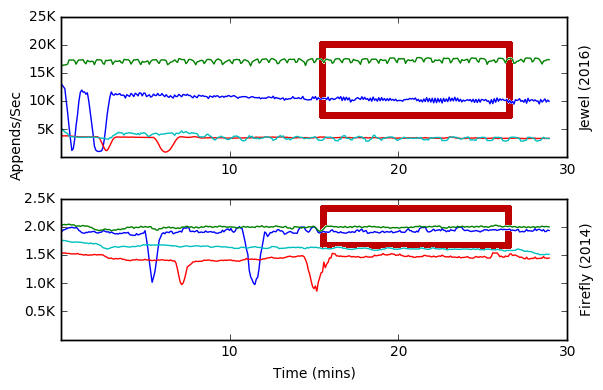
\includegraphics[width=1.0\linewidth]{jewel_v_firefly_pd.png}
        \caption{}
        %\caption{Relative performance differences can be drastic after a software
        %upgrade of the underlying storage system.}
        \label{fig:phy-design}
    \end{subfigure}
    \begin{subfigure}[b]{.33\linewidth}
        \centering
        \includegraphics[width=1.0\linewidth]{batching.png}
        \caption{}
        %\caption{Total throughput with and without batching.}
        \label{fig:batching}
    \end{subfigure}
    \begin{subfigure}[b]{.33\linewidth}
        \centering
        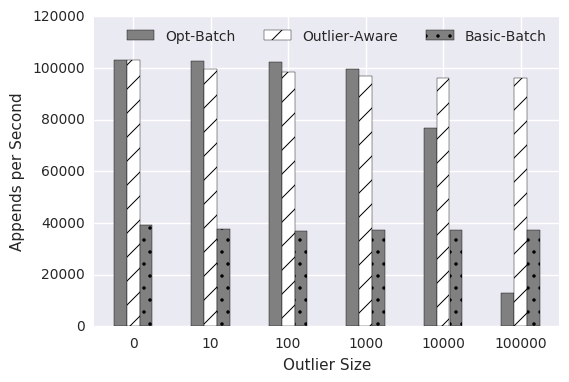
\includegraphics[width=1.0\linewidth]{batching-outlier-detect.png}
        \caption{}
        %\caption{Identifying and handling an outlier independently maintains the
        %beneifts of batching without the performance degredation of unecessarily
        %large I/O requests.}
        \label{fig:batching-outlier}
    \end{subfigure}
    \caption{(a) relative performance differences can be drastic after storage
    software upgrade. (b) total throughput with and without batching.  (c)
    identifying and handling an outlier independently maintains the benefits
    of batching without the performance degradation of unnecessarily large I/O
    requests.}
\end{figure*}

\subsubsection{Application-specific Group Commit}

Group commit is a technique used in database query execution that combines
multiple transactions in order to amortize over per-transaction fixed costs
like logging. Figure~\ref{fig:batching} shows the performance impact of using
a \emph{group commit}-like technique for batching log appends from independent
clients into a single request.  The \emph{Basic-Batch} case implements group
commit at the request level, but processes each sub-request (i.e.  append)
independently using low-level I/O interfaces. The modest performance increase
is attributed to a reduction in average per-request costs related to network
round-trips. Compared with the \emph{Basic-Batch} case, the \emph{Opt-Batch}
implementation is able to achieve significantly higher performance by
constructing more efficient I/O requests using range queries and data sieving
techniques~\cite{x} afforded by the low-level I/O interfaces.

The batched execution technique of group commit can significantly increase
throughput, but the story is much more complex. The ability to apply this
technique requires tuning parameters such as adding artificial delays to
increase batch size that will also affect other metrics such as latency.
While the performance impact of application-specific batching is significant,
techniques such as range queries and data sieving are sensitive to outliers
that can occur with buggy or slow clients.

When outliers occur in a batch, naively building large I/O requests can result
in a large amount of wasted I/O.  Figure~\ref{fig:batching-outlier} highlights
this scope of this challenge. The \emph{Basic-Batch} case handles each request
in a batch independently, and while it performs relatively worse than the
other techniques, it is not sensitive to outliers. The \emph{Opt-Batch}
implementation achieves high append throughput, but performance degrades as
the magnitude of the outlier in the batch increases. In contrast, an
\emph{Outlier-Aware} policy applies a simple heuristic to identify outliers
and handle them independently, resulting in only a slight decrease in
performance over the best case.

\textbf{Takeaway:} Choosing the best implementation of a storage interface
depends on the timing of development (Ceph version), the expertise of
programmers and administrators (Ceph features), the tuning parameters and hardware
selection, as well as system-level and application-specific workload changes.
A direct consequence of such a large design space is that engineers are forced
to duplicate efforts when hardware and software characteristics change. This
is bad: it's unnecessary on-going work, and increases the risk of introducing
bugs that in the best case affect a single application, and in monolithic
designs are more likely to cause systemic data loss.

We believe that with a better understanding of application and interface
semantics there are better approaches than hard-coded and hand-tuned
implementations.  An ideal solution to these challenges is an automated system
search of \emph{implementations}---not simply tuning parameters---based on
programmer produced specifications of storage interfaces in a way that is
independent of optimization strategies, and guaranteed to not introduce
correctness bugs. Next we'll discuss a candidate approach using a declarative
language for interface specification.

\section{Declarative Programmable Storage}
\label{sec:prog-model}

\begin{figure*}[t]
\begin{subfigure}{.8\columnwidth}
    \centering
    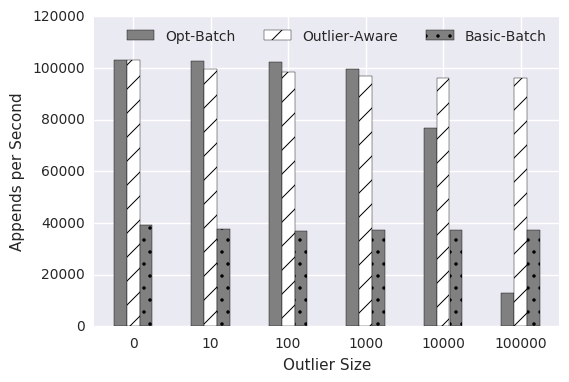
\includegraphics[width=0.95\columnwidth]{batching-outlier-detect.png}
    \caption{}
    %\caption{Identifying and handling an outlier independently maintains the
    %beneifts of batching without the performance degredation of unecessarily
    %large I/O requests.}
    \label{fig:batching-outlier}
\end{subfigure}\hfill
\begin{subfigure}{.3\columnwidth}
\centering
\scalebox{.6}{
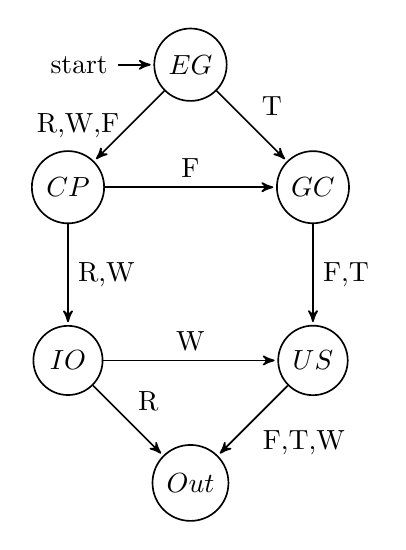
\begin{tikzpicture}[->,>=stealth',shorten >=1pt,auto,node distance=2.2cm,semithick]
%\tikzstyle{every state}=[fill=red,draw=none,text=white]

  \node[initial left,state] (A)              {$EG$};
  \node[state]         (B) [below left of=A] {$CP$};
  \node[state]         (D) [below of=B]       {$IO$};
  \node[state]         (C) [below right of=A] {$GC$};
  \node[state]         (E) [below of=C]       {$US$};
  \node[state]         (F) [below left of=E] {$Out$};

  \path (A) edge        node [left] {R,W,F} (B)
            edge        node {T}     (C)
        (B) edge        node {F}     (C)
            edge        node {R,W}   (D)
        (C) edge        node {F,T}   (E)
        (D) edge        node {W}     (E)
            edge        node {R}     (F)
        (E) edge        node {F,T,W} (F);
\end{tikzpicture}
}
\caption{}
\label{fig:corfu-sm}
\end{subfigure}\hfill
\begin{subfigure}{.65\columnwidth}
\centering
\includegraphics[width=0.95\columnwidth]{Corfu_viz_expanded3.pdf}
\caption{}
\label{fig:dataflow}
\end{subfigure}
\caption{(a) batching performance with and without outlier detection (b) state
machine for the CORFU storage device. (c) logical dataflow of the
CORFU storage protocol which could not be more concise and still capture the
state machine.}
\label{fig:pm}
\end{figure*}

Current ad-hoc approaches to programmable storage restrict
use to developers with distributed programming expertise, knowledge of the
intricacies of the underlying storage system and its performance model, and
use hard-coded imperative methods. This limits the use of optimizations that
can be performed automatically or derived from static analysis.  Based on the
challenges we have demonstrated stemming from the dynamic nature and large
design space of programmable storage, we propose an alternative, declarative
programming model which reduces the learning curve for new users, and allows
existing developers to increase productivity by writing fewer, more portable lines of code.

The model we propose corresponds to a subset of Bloom, a
declarative language for expressing distributed programs as an unordered set
of rules~\cite{alvaro:cidr11}. Bloom rules fully specify program semantics and
allow developers to ignore the details associated with program
evaluation. This level of abstraction is attractive for building storage
interfaces whose portability and correctness is critical. We use Bloom to model the
storage system state uniformly as a collection of relations, with interfaces
expressed as a collection of \emph{queries} over a request stream that
are filtered, transformed, and combined with other system state. We present a
brief example of the CORFU shared-log interface expressed using this model.

\paragraph*{Example: CORFU as a Query}

We model the storage interface of the CORFU protocol as a query in our
declarative language in which the shared-log and metadata are represented by
two persistent abstract collections mapped onto physical storage. This
transformation permits optimizations and implementation details (e.g. log
striping and partitioning) to be discovered and applied transparently by an
optimizer.  Since the specification of the interface is invariant across
system changes and low-level interfaces, the optimizer can automatically
render execution decisions and build indexes using the performance
characteristics of specific access methods.  For example a low-level indexing
engine for text will likely be out-performed by other engines for the CORFU
64-bit write-once address space interface.  Likewise, an instance of the
interface that uses fixed log entries can directly map log entries onto a
low-level byte stream, avoiding an explicit index in some situations.

Amazingly, the semantics of the entire storage interface requirements in
CORFU\footnote{Due to space limitations refer to \cite{watkins:ucsc-soe-16-12}
for a full program listing.} are expressible using only a few Bloom code
snippets amenable as input to an optimizer.  Figure~\ref{fig:corfu-sm}
shows the state transition diagram for the CORFU storage interface and
Figure~\ref{fig:dataflow} shows the corresponding dataflow diagram for the
Bloom CORFU protocol. Beyond the convenience of writing less code, the
entire experience of designing and writing an interface such as CORFU in a
declarative language such as Bloom eases the process of constructing
convincingly correct implementations. Specifically, the high-level details
of the implementation mask distracting issues related to the physical
design and the many other ``gotchas'' associated with writing low-level
systems software.

Our current Bloom specification of CORFU assumes the existence of
an external sequencer service to assign log positions. However, we are working
towards a specification that defines the sequencer service as a view over the
log, whose state is managed in volatile storage. A declarative specification
will be critical to providing portability of the service, since storage
systems internally utilize volatile storage in many forms (e.g. memory caches
and non-replicated data). For example, our work in Malacology showed how inode state in a
distributed file system could be used to build a sequencer,
but an object-based storage system could place sequencer
state in an object cache while providing fast-path access that is difficult to
achieve with the consistency and durability requirements of non-volatile
object state.

%In addition, the CORFU interface depends on a trim
%interface to mark unused poritions of the log (shown on lines 10-15) Trimmed
%entries are tracked as unused for reclamation, and implementations may take
%advantage of specific optimizations provided by an index implementation or
%hardware support found in modern non-volatile memories.

%\begin{lstlisting}[caption={Sample \emph{corfu.bloom} program listing}, label=lst:corfublm]
%bloom :corfu do
%  table :epoch, [:epoch]
%  table :log, [:pos] => [:state, :data]
%  scratch :write_op, op.schema
%end
%bloom :write do
%  temp :valid_write <= write_op.notin(found_op)
%  log <+ valid_write{|o| [o.pos, 'ok', o.data]}
%  ret <= valid_write{|o| [o.type, o.pos, o.epoch, 'ok'] }
%  ret <= write_op.notin(valid_write) {|o| ['read-only'] }
%end
%bloom :trim do
%  log <+- trim_op{|o| [o.pos, 'trimmed']}
%  ret <=  trim_op{|o|
%    [o.type, o.pos, o.epoch, 'ok']}
%end
%\end{lstlisting}


%\begin{figure}
%\centering
%\includegraphics[width=0.7\columnwidth]{Corfu_viz_expanded2.png}
%\caption{Dataflow graph for the CORFU interface written in Bloom}
%\label{fig:flow}
%\end{figure}


%For reference our prototype implementation of CORFU in Ceph (called
%ZLog\footnote{https://github.com/noahdesu/zlog}) is written in C++ and the
%storage interface component comprises nearly 700 lines of code, and uses a
%hard-coded indexing strategy that has been rewritten multiple times to explore
%alternative optimization techniques.

%\begin{figure}[t]
%\begin{subfigure}{.2\columnwidth}
%\centering
%\scalebox{0.4}{
%\begin{tikzpicture}[->,>=stealth',shorten >=1pt,auto,node distance=2.2cm,semithick]
%%\tikzstyle{every state}=[fill=red,draw=none,text=white]
%
%  \node[initial left,state] (A)              {$EG$};
%  \node[state]         (B) [below right of=A] {$CP$};
%  \node[state]         (D) [right of=B]       {$IO$};
%  \node[state]         (C) [above right of=A] {$GC$};
%  \node[state]         (E) [right of=C]       {$US$};
%  \node[state]         (F) [below right of=E] {$Out$};
%
%  \path (A) edge        node [left] {R,W,F} (B)
%            edge        node {T}     (C)
%        (B) edge        node {F}     (C)
%            edge        node {R,W}   (D)
%        (C) edge        node {F,T}   (E)
%        (D) edge        node {W}     (E)
%            edge        node {R}     (F)
%        (E) edge        node {F,T,W} (F);
%\end{tikzpicture}
%}
%\caption{}
%\label{fig:corfu-sm}
%\end{subfigure}\hfill
%\begin{subfigure}{.6\columnwidth}
%\centering
%\includegraphics[width=1.0\columnwidth]{Corfu_viz_expanded.png}
%\caption{}
%\label{fig:malacologyx}
%\end{subfigure}
%\end{figure}

%\begin{figure*}[t]
%\begin{subfigure}{.3\columnwidth}
%\centering
%\scalebox{0.45}{
%\begin{tikzpicture}[->,>=stealth',shorten >=1pt,auto,node distance=2.2cm,semithick]
%%\tikzstyle{every state}=[fill=red,draw=none,text=white]
%
%  \node[initial left,state] (A)              {$EG$};
%  \node[state]         (B) [below right of=A] {$CP$};
%  \node[state]         (D) [right of=B]       {$IO$};
%  \node[state]         (C) [above right of=A] {$GC$};
%  \node[state]         (E) [right of=C]       {$US$};
%  \node[state]         (F) [below right of=E] {$Out$};
%
%  \path (A) edge        node [left] {R,W,F} (B)
%            edge        node {T}     (C)
%        (B) edge        node {F}     (C)
%            edge        node {R,W}   (D)
%        (C) edge        node {F,T}   (E)
%        (D) edge        node {W}     (E)
%            edge        node {R}     (F)
%        (E) edge        node {F,T,W} (F);
%\end{tikzpicture}
%}
%\caption{}
%\label{fig:corfu-sm}
%\end{subfigure}\hfill
%\begin{subfigure}{.5\columnwidth}
%\centering
%\includegraphics[width=0.95\columnwidth]{Corfu_viz_expanded.png}
%\caption{}
%\label{fig:malacologyx}
%\end{subfigure}\hfill
%\begin{subfigure}{0.9\columnwidth}
%
%\begin{lstlisting}[title={{\bf (c)}}, label=lst:write]
%bloom :write do
%  temp :valid_write <= write_op.notin(found_op)
%  log <+ valid_write{ |o| [o.pos, 'valid', o.data]}
%  ret <= valid_write{ |o|
%    [o.type, o.pos, o.epoch, 'ok'] }
%  ret <= write_op.notin(valid_write) {|o|
%    [o.type, o.pos, o.epoch, 'read-only'] }
%end
%\end{lstlisting}
%\end{subfigure}
%\caption{foo}
%\end{figure*}


\section{Discussion and Conclusion}
\label{sec:opts}

It's clear that storage systems are currently in the midst of significant
change and there are few guide posts available to developers navigating a
large and complex design space. This has served as the primary source
of motivation for our use of declarative languages. And while our
implementation does not yet map a declarative specification on to a particular
physical design, the specification provides a powerful infrastructure for
automating this mapping and achieving other optimizations.
Given the declarative nature of the interfaces we have defined, we can draw
parallels between the physical design challenges described in this paper and
the large body of mature work in query planning and optimization.  The Bloom
language that we use as a basis for a declarative specification
produces a dataflow graph that can be used in static analysis, and we
envision that this graph will be made fully available to the storage system to
exploit before and during runtime.

We are currently considering the scope of optimizations that are possible with
such a dataflow model in the context of the storage systems. For instance, without
semantic knowledge of an interface, batching techniques described in
Section~\ref{software} are limited to optimizations such as selecting magic
values for timers and buffer sizes. Semantic information expands the design
space, permitted intelligent reordering or coalescing that depends on
relationships between operations, going beyond what auto-tuning has
previously considered.

{\bf Conclusion.} Optimizing every new or changed application as storage
systems evolve is obviously impractical.  A storage system is not the same as a
database system, but techniques from database optimization can potentially be
leveraged to address complexity, performance and transparent portability for
applications running on evolving storage systems.  Generalizing from the
example we described, we think this approach is innovative and promising. 

%{\bf Conclusion.} With each new application-specific storage interface one
%must consider that the logical conclusion is a future in which little to no
%distinction exists between storage and database systems; or not. But on the
%road to either future intermediate solutions like the one we have proposed are
%necessary to manage complexity and portability.
%Looking beyond standard forms of optimization decisions that seek to select
%an appropriate mix of low-level I/O interfaces, data structure selection is an
%important point of optimization. For instance in Section~\ref{sec:dspace} we
%showed that using the bytestream for metadata management as opposed to the
%key-value interface offered superior performance. However the unstructured
%nature of the bytestream data model imposes no restrictions on implementation
%or storage layout. Integration of common indexing techniques into an optimizer
%combined with a performance model will allow our CORFU interface to derive
%similar optimizations when appropriate. Similar degrees of freedom can be
%imagined when handling other approaches to implementing the CORFU sequencer
%service. Given its soft-state nature heavy-weight processes that enforce
%durability can be circumvented in favor of shorter code paths that optimize
%for throughput and latency.
%
%
%For
%example today object classes are represented as black boxes from the point of
%view of the OSD execution engine.  Understanding the behavior of an object
%class may allow intelligent prefetching. Another type of analysis that may be
%useful for optimization is optimistic execution combined with branch
%prediction where frequent paths through a dataflow are handled optimistically.



{\footnotesize \bibliographystyle{acm}
\bibliography{refs}}



\end{document}
